\section{Dataset and Methodology}
\label{sec:data}

This section details the creation and composition of our novel dataset, SeeSet V1, and the methodologies employed for data processing and augmentation. We first describe the data collection and curation process in \cref{sec:seeset}, followed by a description of the various data modalities generated in \cref{modalities}.

\subsection{SeeSet V1: A Novel Dataset for In-Flight Visibility Estimation}
\label{sec:seeset}
To address the critical need for a comprehensive and realistic dataset for atmospheric visibility research, we developed SeeSet V1. This novel, publicly available dataset is designed to facilitate the evaluation of visibility estimation models under a wide range of conditions, encompassing both ground-level and in-flight scenarios. SeeSet V1 was meticulously curated to incorporate dynamic views from diverse locations, capturing varied scenery from both ground-based and aerial perspectives.

\subsubsection{Dataset Collection and Curation}
\label{data_collection}

To generate our synthetic dataset, we utilized an FAA-approved flight simulator. This advanced simulator facilitates the controlled acquisition of images, showcasing diverse viewpoints and a range of visibility degradations. The process, as illustrated in Figure~\ref{fig:data_collection_process}, starts at ground-level altitude. We systematically increased visibility in incremental steps, extending up to 100 miles. Subsequently, when the visibility reaches its limit, we elevate the viewpoint's altitude and then reset the visibility to 0, repeating this procedure up to a maximum of 2000 feet AGL.

\begin{figure}[htbp]
\centerline{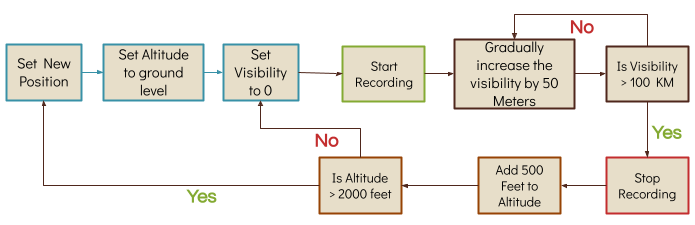
\includegraphics[width=250pt]{imgs/data_collection_pipeline.png}}
\caption{Dataset Collection Process}
\label{fig:data_collection_process}
\end{figure}
 
The collected images are automatically labeled into five discrete bins, each tailored to specific \href{https://www.faa.gov/air_traffic/publications/atpubs/aim_html/}{FAA requirements}. This categorization is based on visibility conditions and regulations relevant to both ground-based and aerial environments. The designated bins serve as the basis for the five labels utilized in training our DL models. We report the classes (bins) specifications and the corresponding counts in Table~\ref{tab:vis_img_count}.

\begin{figure*}
    \centering
    \subfigure[Bin 0]{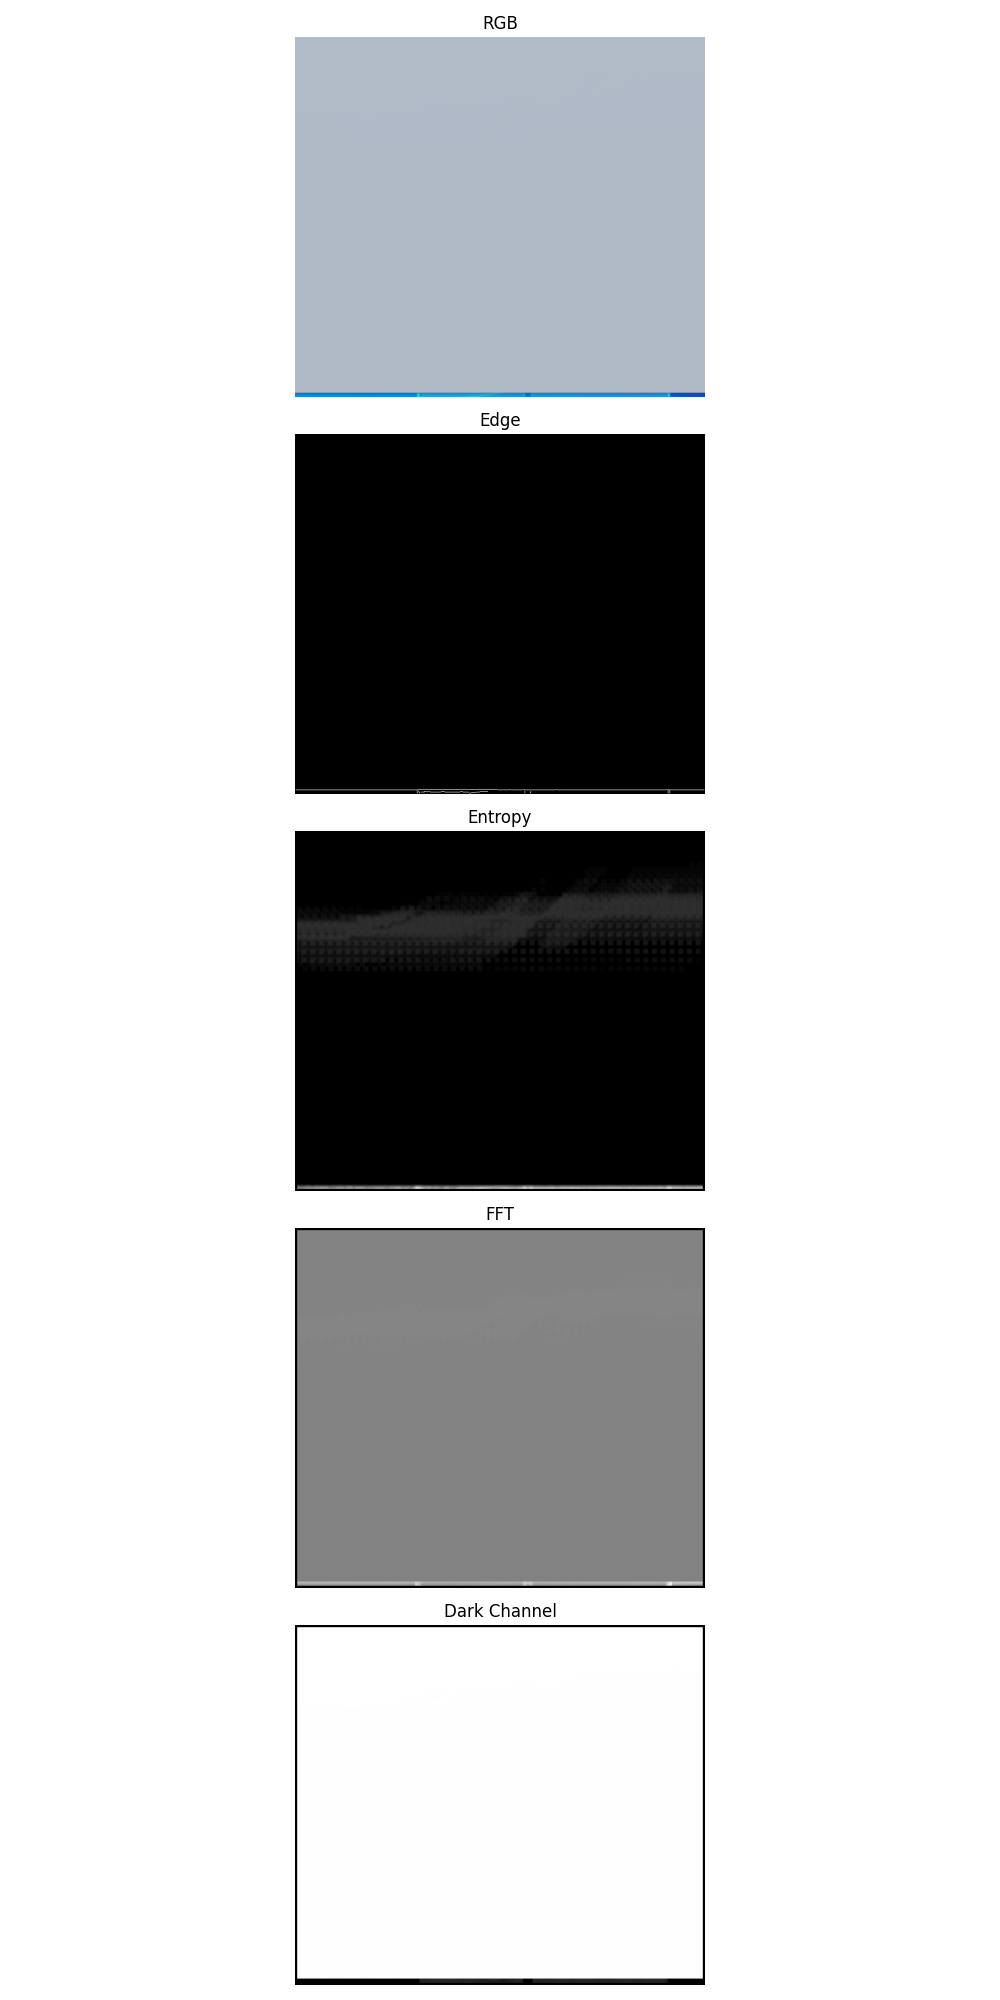
\includegraphics[width=0.14\textwidth, trim={7.5cm 0 7.5cm 0},clip]{imgs/examples/exp_0_featuresMiles_0.12427454732996136_featuresM_200_features.png}\label{subfig:bin0}}
    \subfigure[Bin 1]{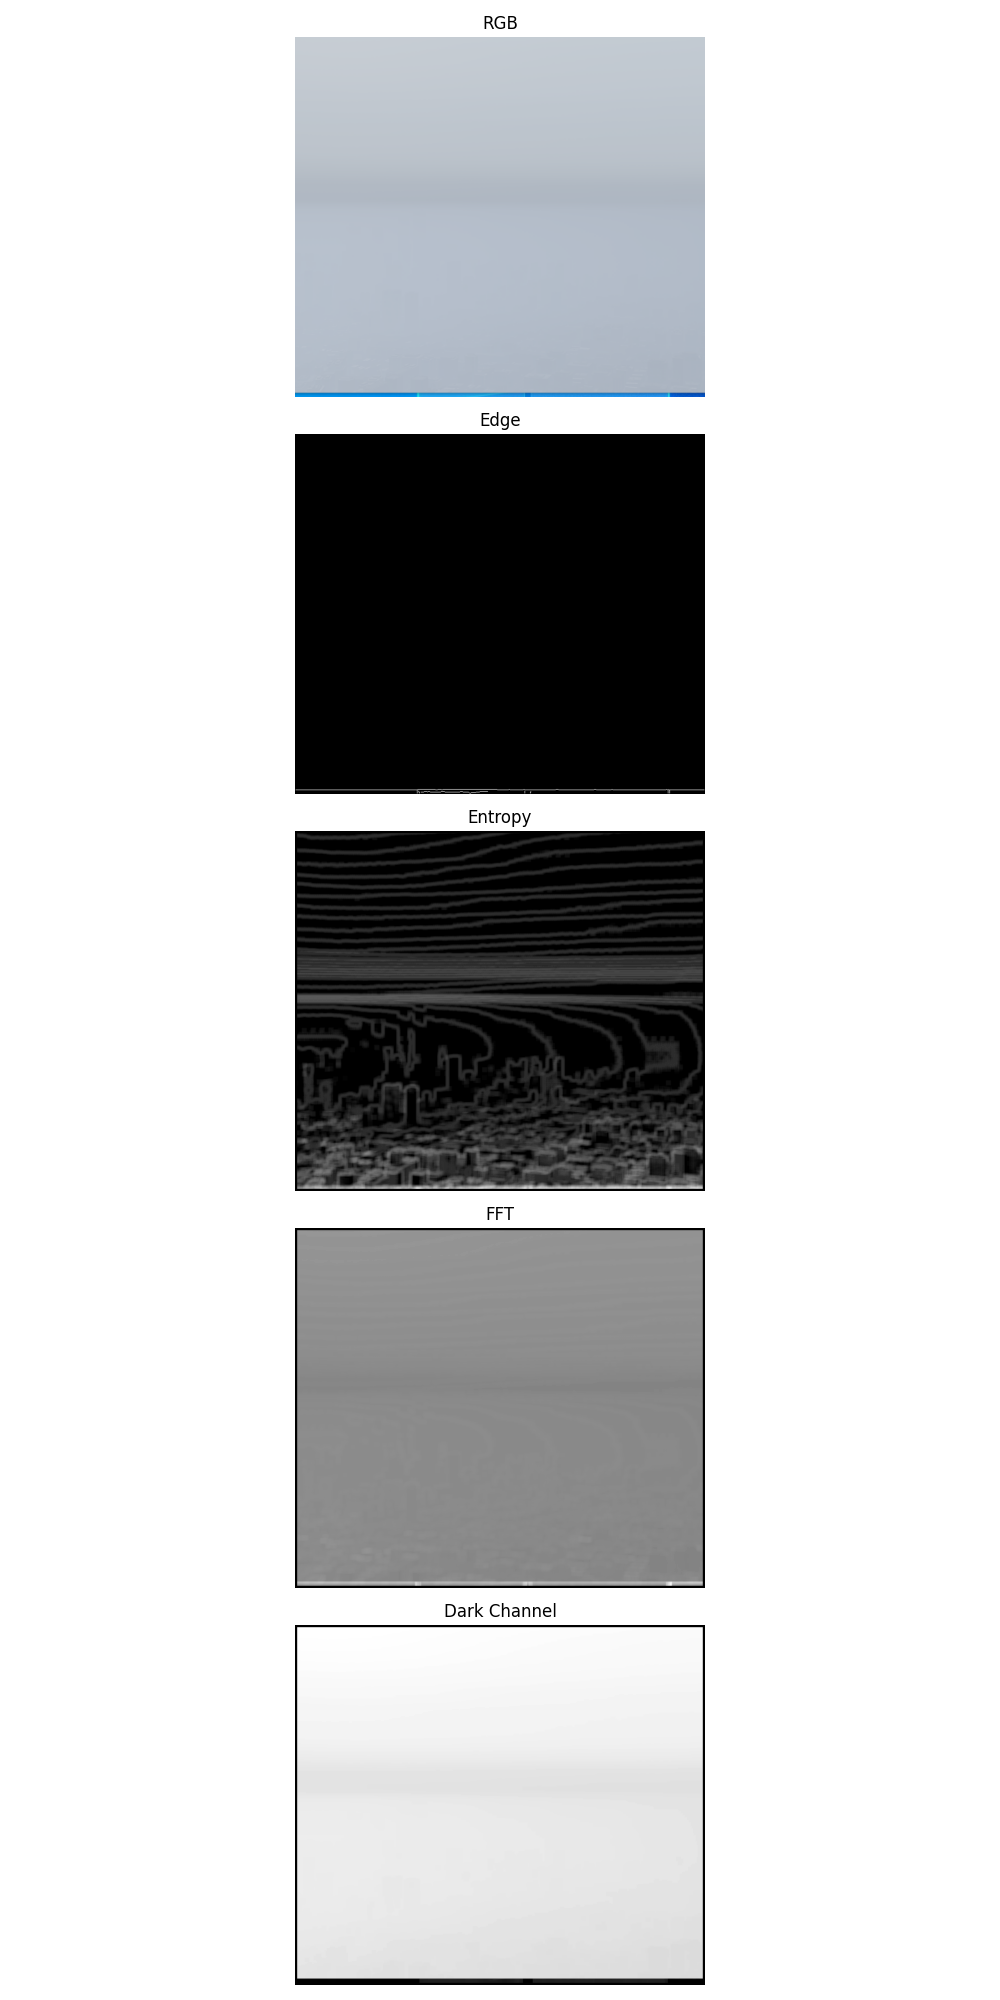
\includegraphics[width=0.14\textwidth, trim={7.5cm 0 7.5cm 0},clip]{imgs/examples/exp_0_featuresMiles_0.9320591049747102_featuresM_1500_features.png}\label{subfig:bin1}}
    \subfigure[Bin 2]{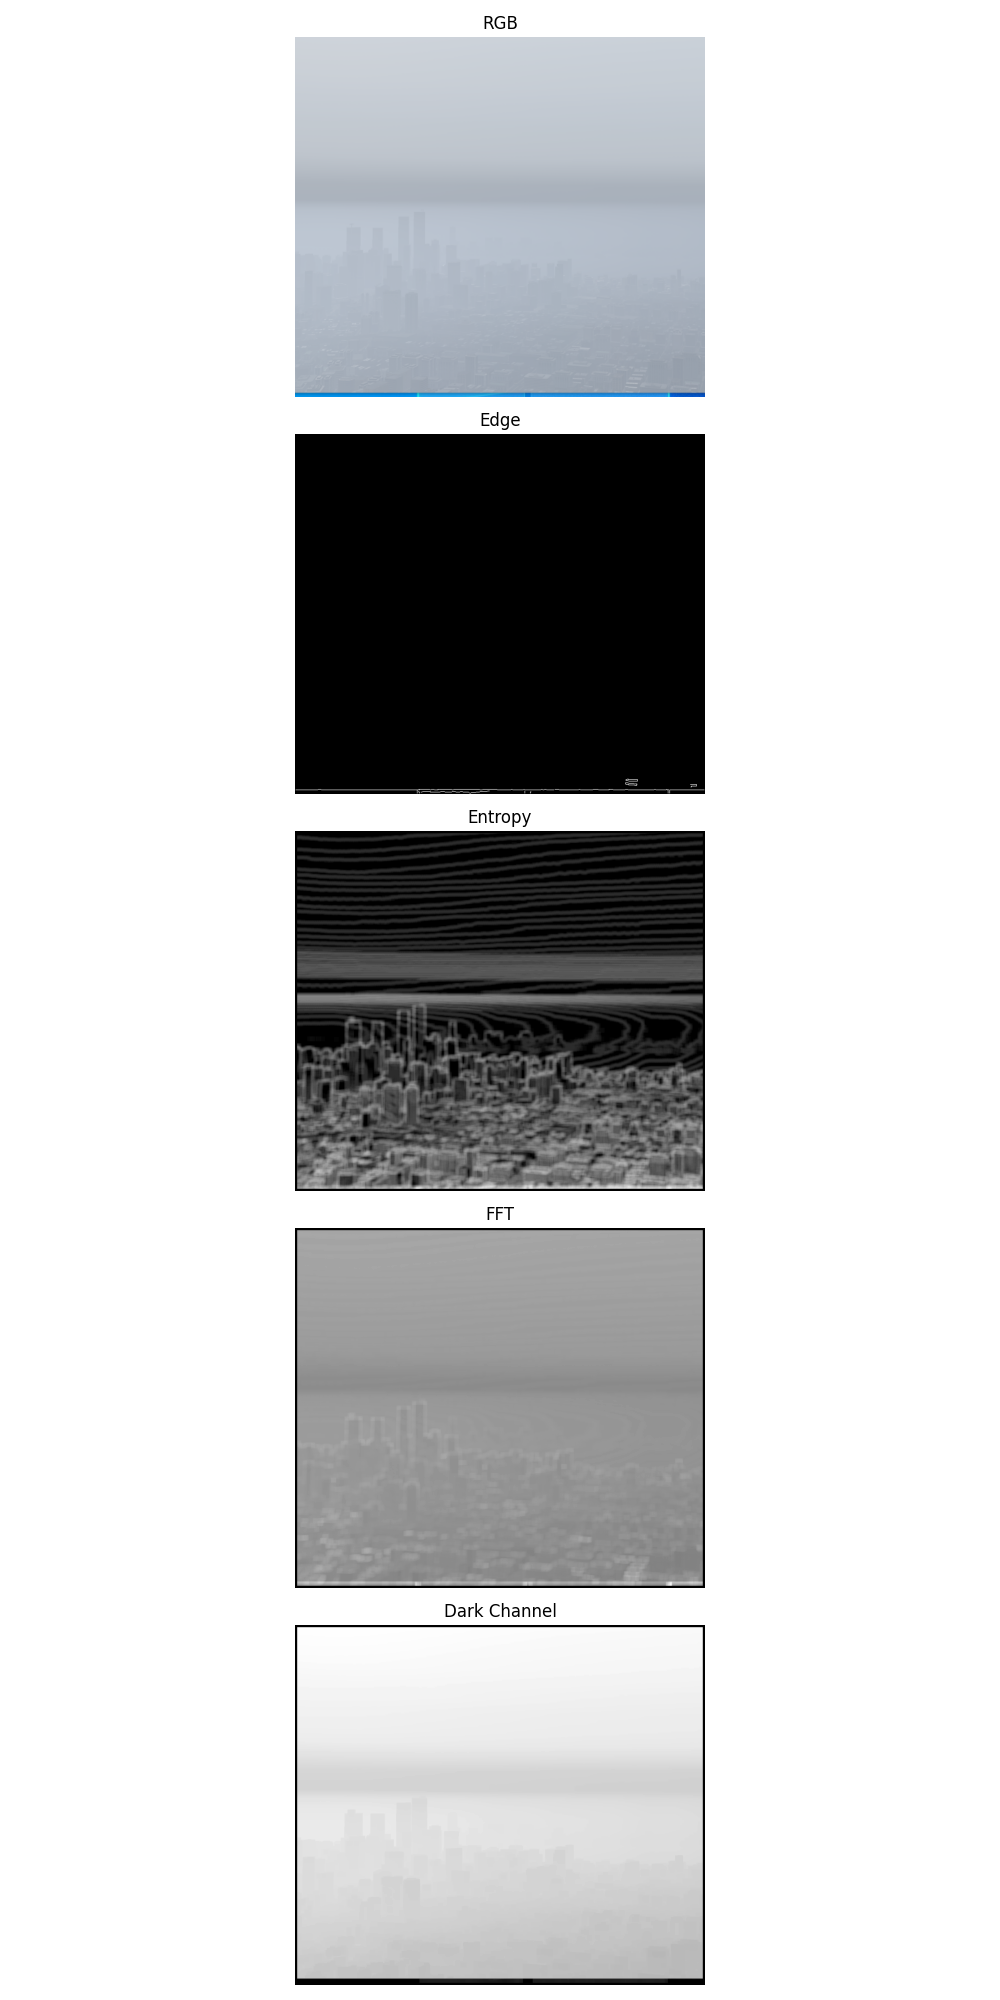
\includegraphics[width=0.14\textwidth, trim={7.5cm 0 7.5cm 0},clip]{imgs/examples/exp_0_featuresMiles_1.8951868467819106_featuresM_3050_features.png}\label{subfig:bin2}}
    \subfigure[Bin 3]{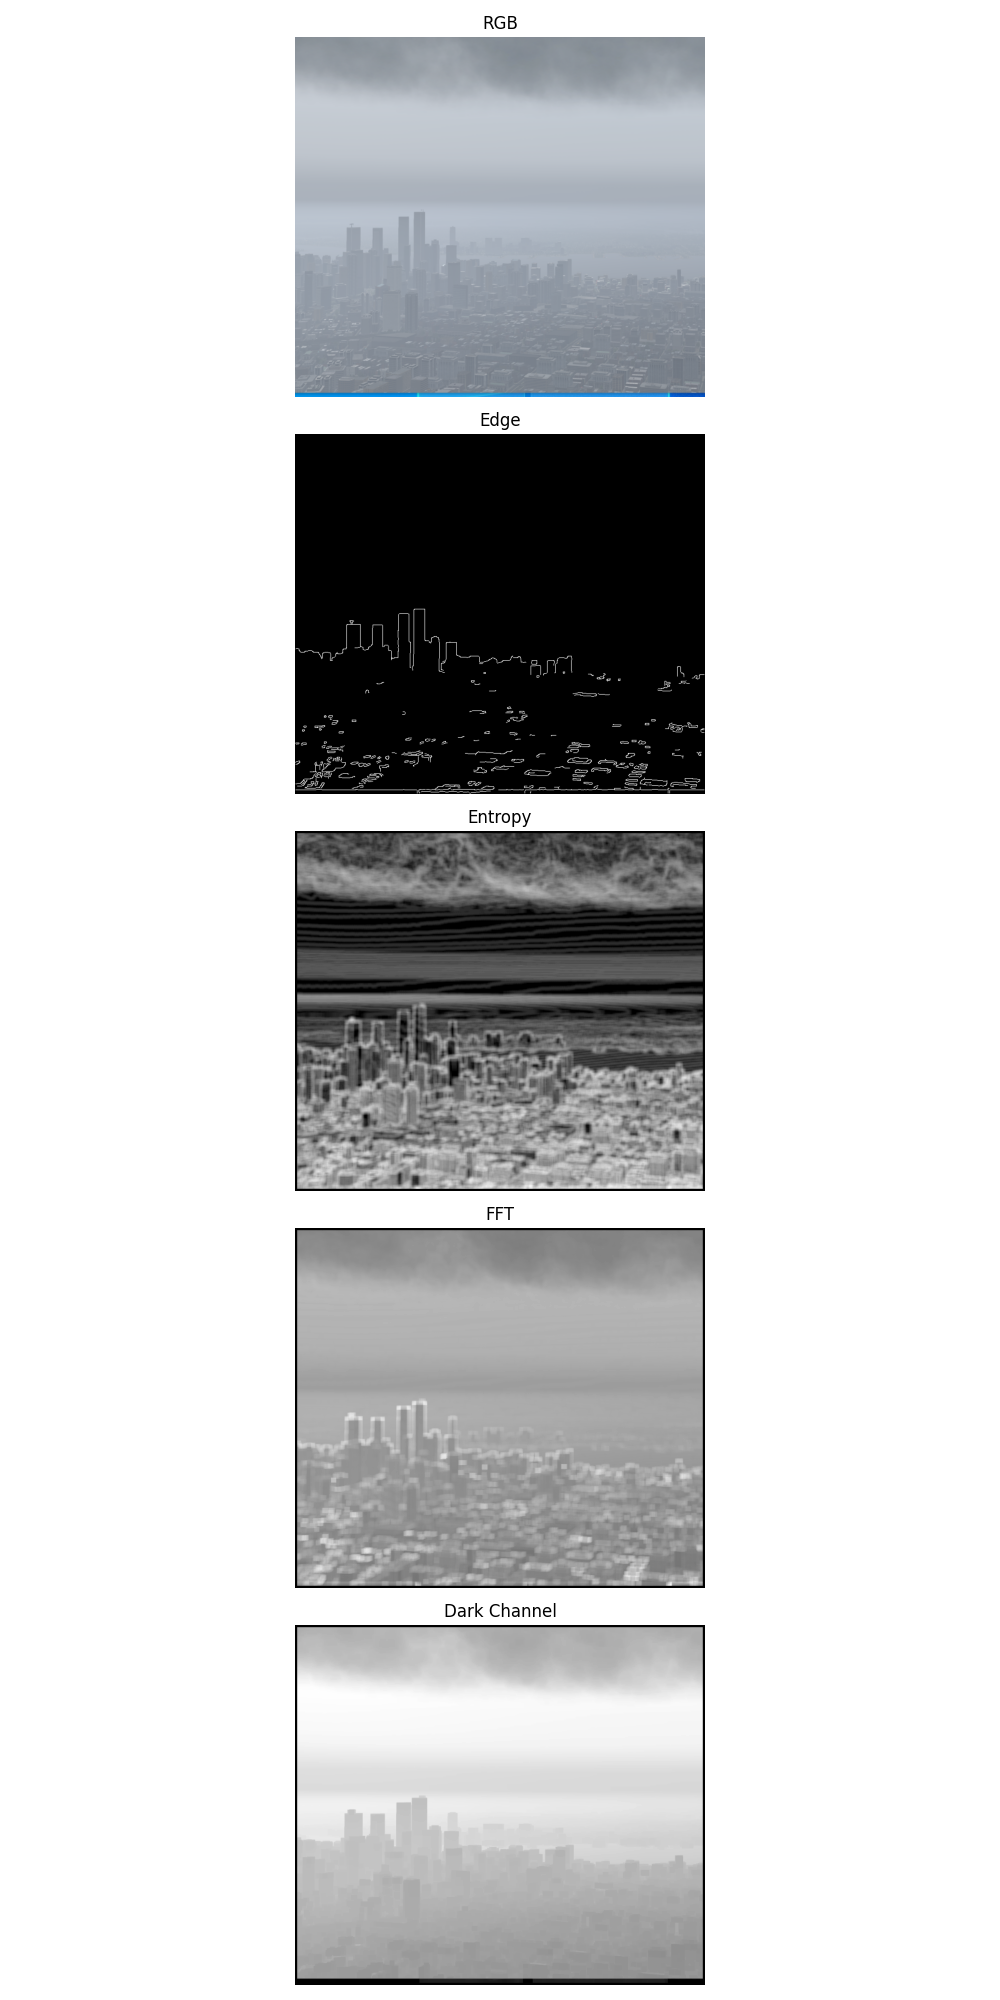
\includegraphics[width=0.14\textwidth, trim={7.5cm 0 7.5cm 0},clip]{imgs/examples/exp_0_featuresMiles_4.038922788223744_featuresM_6500_features.png}\label{subfig:bin3}}
    \subfigure[Bin 4]{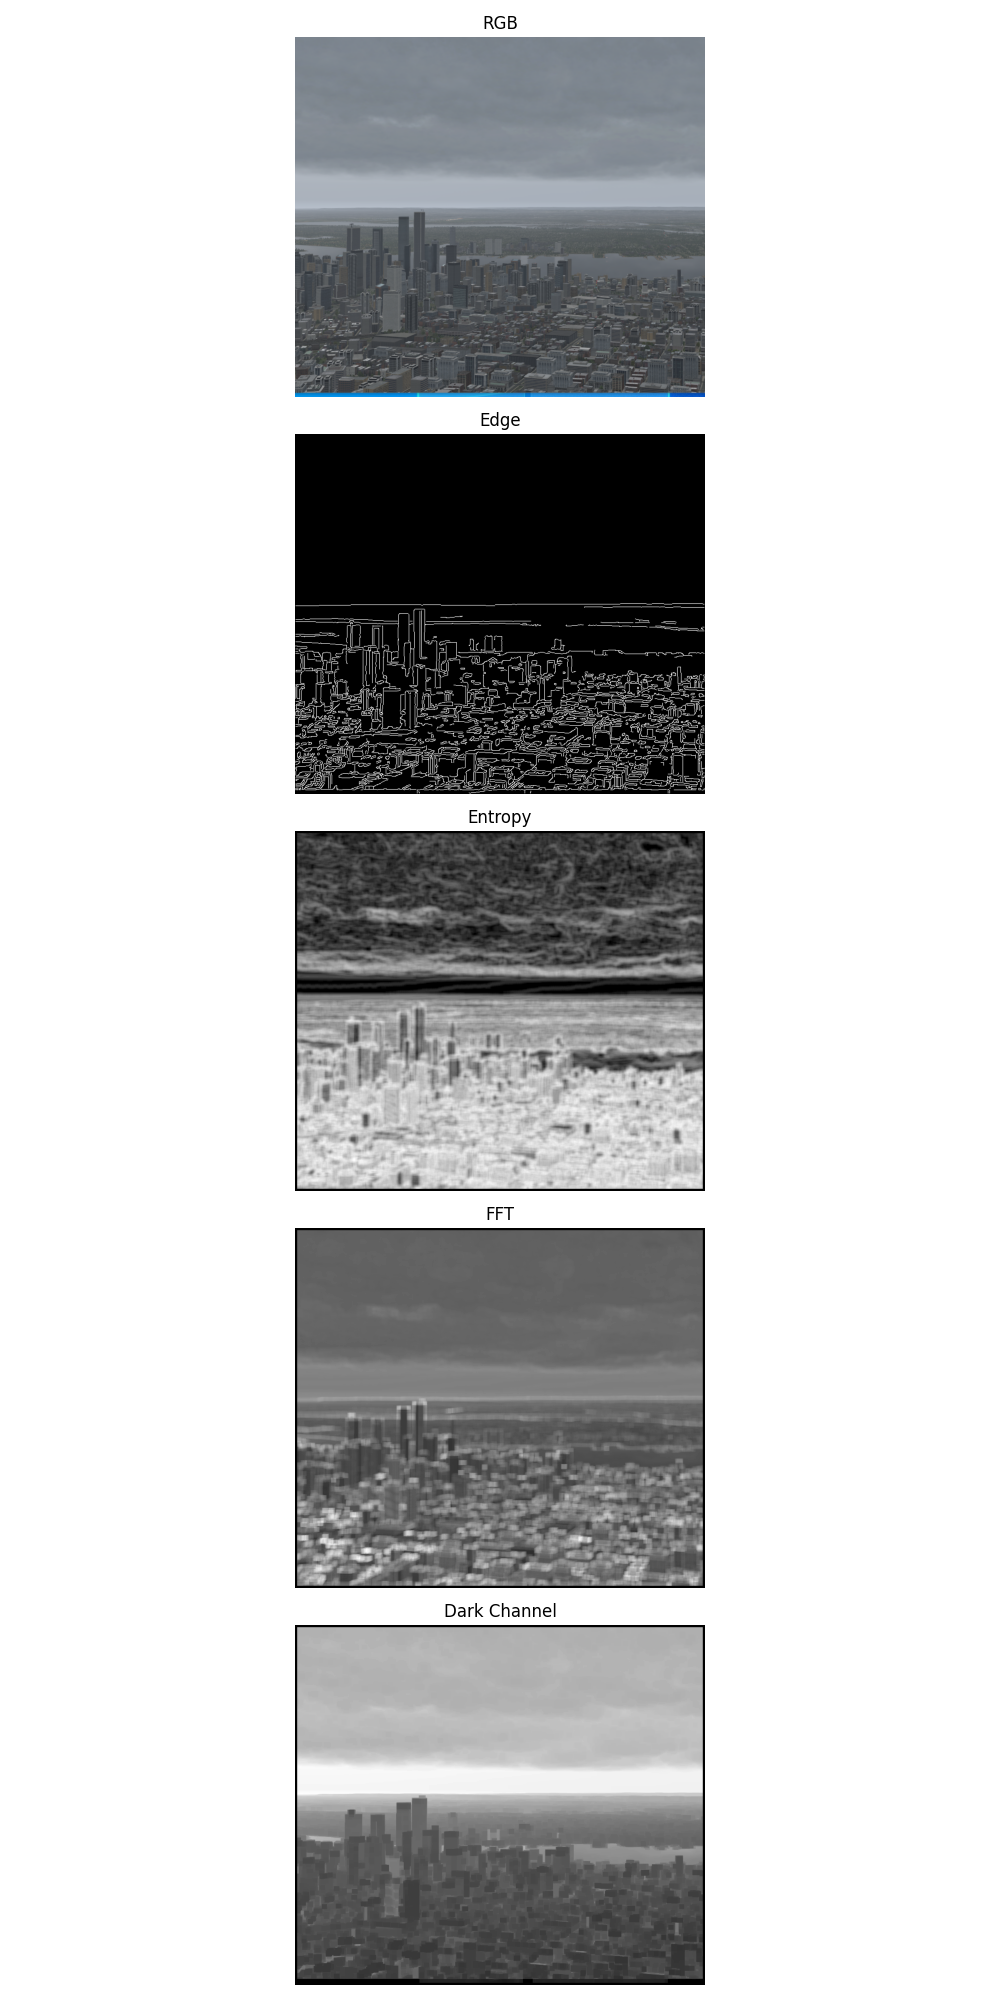
\includegraphics[width=0.14\textwidth, trim={7.5cm 0 7.5cm 0},clip]{imgs/examples/exp_0_featuresMiles_46.1462462872979_featuresM_74265_features.png}\label{subfig:bin4}}
    \caption{Examples from SeeSet V1 showing the impact of visibility on RGB images for the 6N7 Sealane 01 View. Each column corresponds to a different visibility bin: (a) $< 0.5$ miles, (b) $(0.5, 1]$ miles, (c) $(1, 3]$ miles, (d) $(3, 5]$ miles, and (e) $> 5$ miles.}
    \label{fig:impact_vis_deg_features}
\end{figure*}

Diversity in a DL benchmark dataset is crucial for robust model training and evaluation. Including a comprehensive range of visibility scenarios, such as different land covers and various times of the day, ensures that the dataset reflects real-world variability. This diversity allows DL models to learn and generalize well across different conditions, making them more capable of handling a wide range of scenarios when deployed in practical applications.

\begin{table}[htbp]
\centering
\caption{Visibility Categories and Image Counts in SeeSet V1}
\label{tab:vis_img_count}
\begin{tabular}{@{}lccr@{}}
\toprule
\textbf{Category} & \textbf{Visibility (miles)} & \textbf{Visibility (meters)} & \textbf{Count} \\
\midrule
4 & $\geq$ 5 & $\geq$ 8046.72 & 67,002 \\
3 & 3 to 5 & 4828.03 to 8046.72 & 19,584 \\
2 & 1 to 3 & 1609.34 to 4828.03 & 19,648 \\
1 & 0.5 to 1 & 804.672 to 1609.34 & 4,928 \\
0 & $\leq$ 0.5 & $\leq$ 804.672 & 4,938 \\
\midrule
\textbf{Total} & & & \textbf{116,100} \\
\bottomrule
\end{tabular}
\end{table}

\subsubsection{Data Modalities}
\label{modalities}

In addition to RGB images, we generate several other data modalities to provide richer information for visibility estimation. These modalities are described below.

\paragraph{Monocular Depth Estimation}
We utilize the Omnidata toolkit to extract depth maps from monocular images \cite{eftekhar2021omnidata}. This toolkit provides a scalable method for depth estimation, essential for understanding the spatial arrangement in a scene. The generated depth maps offer a pixel-wise measurement of distance from the viewpoint, aiding in the accurate representation of the three-dimensional structure of the scene. A notable limitation of the depth estimation model is that it was trained to mask the sky, which may affect performance on our images collected at various altitudes.

\paragraph{Normal Surface Estimation}
Alongside depth maps, we also employ the Omnidata toolkit for normal surface estimation \cite{eftekhar2021omnidata}. This modality provides information about the orientation of surfaces in the image, which is crucial for understanding the geometric properties of the scene. Unlike the depth estimator, this model considers both sky and ground details.

\paragraph{Entropy Map}
We incorporate an image entropy map as a modality to enhance the model's sensitivity to changes in visibility, especially in low-visibility conditions. The entropy map quantifies the amount of information present in different regions of an image. The procedure to generate the Entropy Maps is detailed in Algorithm \ref{alg:entropy_map}.

\begin{algorithm}[htbp]
\caption{Calculate Entropy Map}\label{alg:entropy_map}
\begin{algorithmic}[1]
\Require An image $I$ represented as a 2D array, window size $w$
\Ensure Entropy map $E$ of the same dimensions as $I$
\State $E \gets \text{zeros\_like}(I)$ \Comment{Initialize entropy map}
\State $rows, cols \gets$ dimensions of $I$
\For{$i \gets 0$ \textbf{to} $rows - w$}
    \For{$j \gets 0$ \textbf{to} $cols - w$}
        \State $window \gets I[i : i+w, j : j+w]$
        \State $hist \gets \text{calculateHistogram}(window)$
        \State $hist \gets hist / \text{sum}(hist)$
        \State $entropy \gets -\sum (hist \cdot \log_2(hist + \epsilon))$
        \State $E[i + \frac{w}{2}, j + \frac{w}{2}] \gets entropy$
    \EndFor
\EndFor
\State \Return $E$
\end{algorithmic}
\end{algorithm}

\paragraph{Edge Detection}
Edge detection is another key modality well-suited for scenarios involving long-range visibility where the definition of objects and scene boundaries is critical. By highlighting the contours and edges within the images, this modality aids in delineating shapes and structures, thus providing a clear distinction between different objects and features in the scene.

\begin{figure*}[htbp]
    \centering
    \begin{subfigure}[b]{0.24\textwidth}
        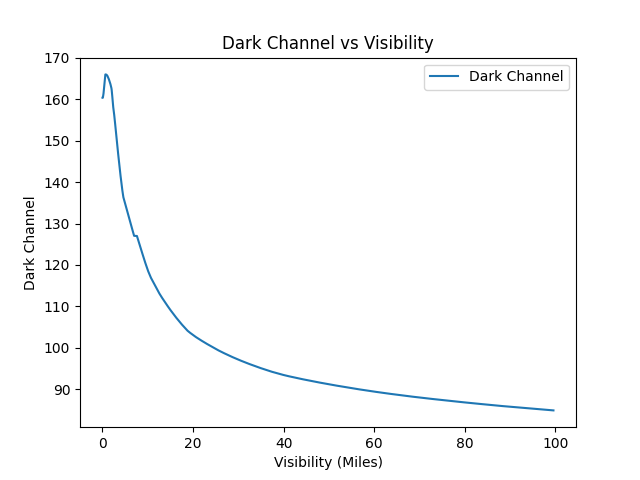
\includegraphics[width=\textwidth]{imgs/dark_channel_vs_visibility.png}
        \caption{Dark Channel Prior}
        \label{fig:mean_dark_channel}
    \end{subfigure}
    \hfill
    \begin{subfigure}[b]{0.24\textwidth}
        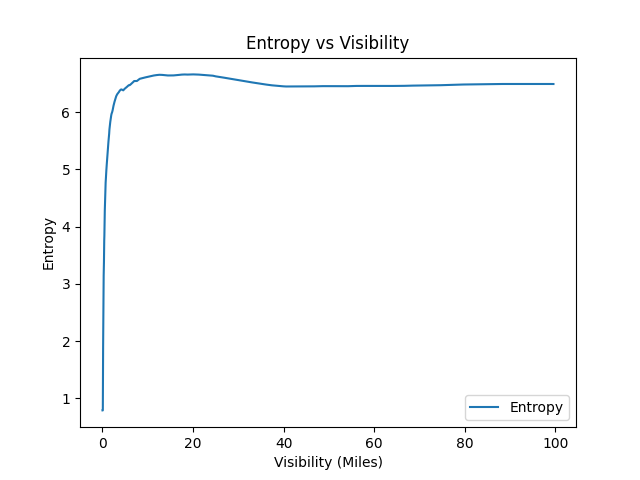
\includegraphics[width=\textwidth]{imgs/entropy_vs_visibility.png}
        \caption{Entropy}
        \label{fig:mean_entropy}
    \end{subfigure}
    \hfill
    \begin{subfigure}[b]{0.24\textwidth}
        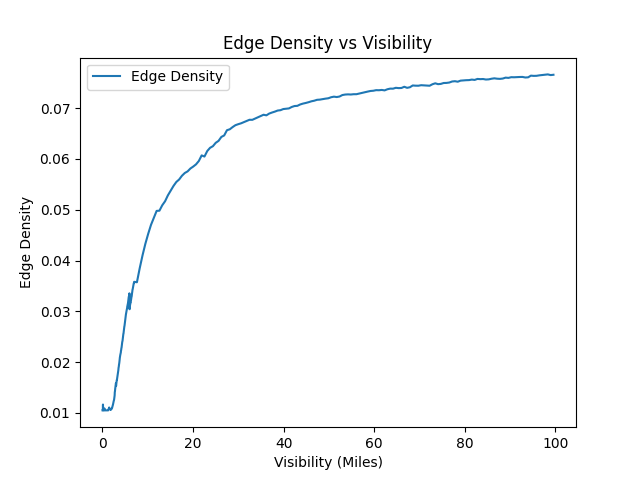
\includegraphics[width=\textwidth]{imgs/edge_density_vs_visibility.png}
        \caption{Edge Density}
        \label{fig:mean_edge_density}
    \end{subfigure}
    \hfill
    \begin{subfigure}[b]{0.24\textwidth}
        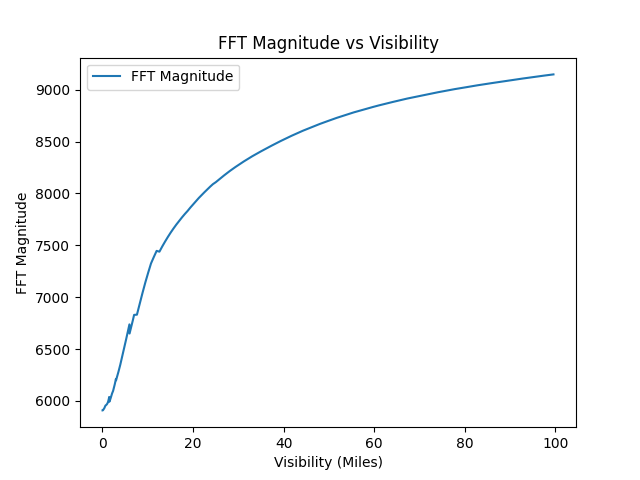
\includegraphics[width=\textwidth]{imgs/fft_magnitude_vs_visibility.png}
        \caption{FFT Magnitude}
        \label{fig:mean_fft}
    \end{subfigure}
    \caption{Impact of Visibility Degradation on Various Image Features. The plots show the mean value of each feature as a function of visibility in miles, demonstrating a clear correlation between the features and the level of visibility.}
    \label{fig:mean_of_features}
\end{figure*}

Figure~\ref{fig:mean_of_features} illustrates the impact of visibility degradation on various image features, showing a clear correlation between these features and visibility levels.